\documentclass[11pt,a4paper]{article}
\usepackage{fontspec}
\setmainfont{chinese.ttf}[Path=fonts/,BoldFont=chinese.ttf,BoldFeatures={FakeBold=1.5},ItalicFont=chinese.ttf,ItalicFeatures={FakeSlant=0.15}]
\XeTeXlinebreaklocale "zh"
\XeTeXlinebreakskip=0pt plus 1pt minus 0.5pt
\renewcommand{\abstractname}{摘要}\renewcommand{\refname}{参考文献}\renewcommand{\figurename}{图}\renewcommand{\tablename}{表}
\usepackage[margin=24mm]{geometry}
\usepackage{amsmath,amssymb,booktabs,tabularx,graphicx,array,placeins}
\usepackage[font=small,labelfont=bf,labelsep=quad]{caption}
\usepackage[colorlinks=true,allcolors=black]{hyperref}
\hypersetup{pdftitle={文献催化机器学习的跨来源泛化差距},
  pdfauthor={Zhang Junyu and Li Wenjie},
  pdfcreator={XeLaTeX}}
\setlength{\parskip}{4pt}
\setlength{\parindent}{2em}
\linespread{1.12}
\emergencystretch=3em
\setcounter{topnumber}{3}\setcounter{bottomnumber}{2}\setcounter{totalnumber}{5}
\renewcommand{\topfraction}{.88}\renewcommand{\bottomfraction}{.8}\renewcommand{\textfraction}{.08}\renewcommand{\floatpagefraction}{.68}
\newcommand{\pp}{\,\text{个百分点}}
\newcommand{\mgg}{\,mg\,h$^{-1}$\,g$_{\mathrm{cat}}^{-1}$}

\title{\textbf{文献催化机器学习的跨来源泛化差距：\\
少标签适配、输入表征与公开研究复核}}
\author{张君宇\quad 李文杰\\[2pt]
\small 中国石油大学（华东）机电工程学院，青岛 266580}
\date{2026年9月28日}


\begin{document}
\maketitle
\begin{abstract}
\noindent
从不同文献汇编的催化数据往往带有各自的实验与报告特点。因此，需要分别回答两个问题：随机划分实验记录得到的成绩，能否代表对陌生文献来源的预测能力；获得少量新来源的真实实验结果后，预测又能改善多少。
本文建立按文献来源隔离训练与测试、控制标签数量、在同一来源内配对比较并加入负对照的评估框架。“标签”指一条记录的实测结果；利用少量新来源标签调整预测，称为少标签适配。
研究覆盖两个反应体系、四个预测目标，包括1,245条同时报告甲醇转化率与选择性的记录、1,230条甲醇时空收率（STY）记录，以及1,794条甲烷氧化偶联（OCM）记录。
将具有共同来源或重复关系的记录整体留出后，四个目标的合并决定系数$R^2$相对于记录随机划分下降0.20--0.47。
提供五条新来源标签可明显降低部分任务的误差：在基础评估中，局部岭回归将甲醇转化率的来源等权平均绝对误差（MAE）由5.279降至2.429\pp{}。
配对的输入信息比较和标签置换分析，进一步区分了“获知来源整体水平”与“利用正确的条件--结果对应关系”两类收益；局部、残差及组合模型则用于检查历史预测结构的额外作用。
在均提供五条标签、保持组合预测模型配置相同的条件下，面向待预测记录的V最优选样将STY的MAE由62.608降至50.274\mgg{}，将OCM工况加组成设置（F1）的MAE由3.081降至2.708\pp{}，分别降低19.7\%和12.1\%；两项均通过原定五项任务的多重比较校正。
91个额外文献来源和一个包含1,739条测量的作者实测实验家族扩大了验证范围；在该家族的20次催化剂编号分离划分中，组成信息引导的选样有19次改善预测。
两项公开研究的原流程结果均可在各自口径下恢复。来源隔离复核中，Suvarna受控比较的$R^2$由0.876降至0.319；Xu后续相同五折的配对比较中，来源等权MAE由69.620升至126.365，单位为原始STY单位。
这些结果将跨来源预测差距、少量实测结果的利用、输入信息与测量覆盖，以及公开研究的评估范围连接起来，为有限标签条件下的催化预测提供可复核的依据。
\end{abstract}

\section{引言}
催化机器学习常使用从已发表文献中汇编的数据。每篇论文提供的测量数量有限，并带有其催化剂制备、表征方法、原料纯度和报告习惯的特点。TheMeCat\cite{toldy}、三十年甲醇合成回顾\cite{yan}、Suvarna等的时空收率数据集\cite{suvarna}和Schmack等的氧化偶联荟萃分析\cite{schmack}为这类研究提供了基础，相关模型也经常报告较高的预测成绩。

\paragraph{两种划分回答不同的预测问题。}
如果把所有实验记录混合后随机划分，同一篇论文的部分记录可能用于训练，另外部分用于测试。这样的评价考察的是：模型能否预测已经接触过的来源中的其他记录。同一论文的记录往往共享装置、催化剂族和报告方式，部分训练与测试记录也可能非常接近。
对于此前完全没有见过的文献来源，则需要将该文献的记录整体留作测试；具有相同上游测量或共同引用关系的记录，也应一起划分。本文将这一做法称为来源隔离评估。
域适应理论说明，仅有训练来源上的较好表现，不足以约束新来源上的误差\cite{bendavid}；对存在分组结构的数据采用分组重采样，也是已有的标准做法\cite{roberts}。催化研究仍需要跨反应体系、跨预测目标量化两类评价的差距，并检验可行的改善方式。

\paragraph{用少量新来源结果帮助预测。}
面对新来源，可以先获得其中少量记录的真实结果，再用这些结果调整对其余记录的预测。本文把实测结果称为标签，把这一过程称为少标签适配；输入则是事先已知的工况、组成等信息。
均值偏移、带正则化的仿射校正、经验贝叶斯收缩\cite{efron}和局部回归都是已有方法，多元校准迁移在化学计量学中也有长期积累\cite{feudale}。
本文关注的是如何可靠地比较这些方法：每次允许获得多少条结果，与哪些简单而有竞争力的方法比较，以及收益在不同来源之间是否一致。文中的“标签预算”仅表示允许提供的结果条数，不表示已经计算出实验经费，也不保证每条文献记录对应一次相互独立的实验。

\paragraph{解释少量标签提供了哪些信息。}
少量新结果可能首先揭示该来源的整体水平。例如，均值偏移可以修正历史模型在该来源上的整体高估或低估。使用输入特征的局部模型还可能学到来源内部的条件--结果关系。
仅比较平均误差，无法区分这两种作用。因此，本文保持已选结果的数值集合和均值不变，打乱它们与输入的配对，检查预测是否变差；再在相同记录和划分上比较不同输入表征。这里的“表征”指提供给模型的信息及其数值编码方式。

\paragraph{在公开研究中核对评估范围。}
为检查上述现象是否局限于本文组织的数据分析，我们还重新运行两项数据和代码公开的已发表研究，并对它们进行来源隔离评价。原流程能否复现，与原流程成绩能否代表陌生来源预测能力，分别检验。

\paragraph{本文贡献。}
第一，建立来源隔离、标签数量明确的评估流程，包括固定测试集、逐步增加的支持标签、同来源配对比较和负对照。第二，在两个反应体系、四个目标上量化随机记录划分与来源隔离评价的差距，并报告0、1、2、3、5、10条标签下的表现。第三，区分来源整体水平、正确输入--结果对应关系及输入表征的作用，并通过较强局部模型和相同标签数量下的选样对照检验成立条件。第四，对两项公开工作进行复现与来源隔离复核。
经典估计器和V最优设计本身不作为新算法贡献；本文的重点是把这些问题组织为可检查的催化预测证据链。

\section{相关工作}
对于具有聚类结构的数据，分组或分块重采样已有成熟基础\cite{roberts}；近期催化基准也比较了按化学式分组与随机交叉验证\cite{wu}。域适应理论区分训练来源精度和目标来源误差\cite{bendavid}。
本文采用的适配方法同样有明确的既有基础：均值偏移和仿射再校准属于标准实践\cite{steyerberg2019}，经验贝叶斯收缩可追溯至Efron与Morris\cite{efron}，多元校准迁移已有化学计量学综述\cite{feudale}。
主要数据来自TheMeCat\cite{toldy}、\emph{Communications Engineering}甲醇回顾\cite{yan}、Schmack等的OCM荟萃分析\cite{schmack}和Suvarna等的STY研究\cite{suvarna}。这些数据工作未将“明确限制可用新标签数量的来源隔离评价”作为主要协议。相关定位与原协议细节见补充材料A。

\section{数据}\label{sec:data}
\subsection{数据来源与预测目标}
表\ref{tab:data}列出四个目标的数据与来源数量。甲醇转化率和选择性共用1,245条成对记录，来自82个文献来源、80个防泄漏分组，由TheMeCat v1\cite{toldy}和甲醇回顾数据集\cite{yan}组合而成。
甲醇STY数据来自Suvarna等的公开数据集\cite{suvarna}，包含1,230条记录、109个来源，采用CC BY 4.0许可；其中20个出版物标识与转化率数据重叠，因此将其视为同一反应体系中的另一个预测目标。
OCM数据来自Schmack等的荟萃分析\cite{schmack}，包含1,794条记录、408个来源、405个防泄漏分组，预测C$_2$收率。
转化率、选择性与C$_2$收率的误差以百分点表示；STY的误差保留其产量单位，不跨目标直接比较数值大小。
\begin{table}[t]
\centering\small
\caption{数据集、预测目标与主要比较来源集合。主队列指在固定测试集之外，仍有足够记录提供最多10条标签、因而可以完成整条标签数量曲线的来源。设某来源有$n$条记录，其固定测试集包含$\max(5,\lceil n/4\rceil)$条。pp表示百分点；STY为单位催化剂质量、单位时间的甲醇产量。}
\label{tab:data}
\begin{tabularx}{\linewidth}{lXXXX}
\toprule
 & CO$_2$转化率 & 甲醇选择性 & 甲醇STY & OCM C$_2$收率 \\
\midrule
记录数 & \multicolumn{2}{c}{1{,}245（成对）} & 1{,}230 & 1{,}794 \\
来源数 & \multicolumn{2}{c}{82} & 109 & 408 \\
泄漏组数 & \multicolumn{2}{c}{80} & 109 & 405 \\
主队列来源数 & \multicolumn{2}{c}{32} & 28 & 22 \\
单位 & \multicolumn{2}{c}{pp} & mg\,h$^{-1}$g$_{cat}^{-1}$ & pp \\
输入信息 & \multicolumn{4}{l}{工况描述符（甲醇另含SBET；OCM F1另含所记录组成）} \\
许可 & \multicolumn{4}{l}{CC BY 4.0（TheMeCat、OCM补充材料、STY数据集）} \\
\bottomrule
\end{tabularx}
\end{table}

\subsection{数据重建与纳入标准}
甲醇数据从两份上游文件逐行重建（表\ref{tab:ledger}）。原始1,124和500行分别保留748和497条成对记录。纳入规则在查看模型表现前固定：转化率和选择性均已报告且位于$[0,100]$；温度、压力和H$_2$/CO$_2$已报告且为正；GHSV与BET允许缺失，并在训练分区内填补。
真实的零响应保留；完全重复的上游记录仅保留一份；即使条件与结果相同，只要组成不同，仍视为不同测量。所有排除原因逐行留档，不依据模型成绩筛选记录。
早期内部版本中有20条BET记录曾按$10^{\mathrm{LN}}$恢复，现根据已存储的自然对数字段改用$\exp(\mathrm{LN})$重算，修正过程保留日志。
OCM数据采用同样的可追溯处理原则：从1,802条原始记录和412个出版物编号出发，排除参考表缺失或归属有歧义的条目，并合并三对引用相同的来源。
\begin{table}[t]
\centering\small
\caption{甲醇数据的纳入与排除记录。每条被排除记录均保留原因；筛选不依据模型表现。}
\label{tab:ledger}
\begin{tabular}{lrr}
\toprule
 & TheMeCat v1 & CommsEng MeOH \\
\midrule
上游文件行数 & 1{,}124 & 500 \\
纳入的成对记录 & 748 & 497 \\
无成对目标 & $-319$ & --- \\
恰缺一条目标 & $-26$ & --- \\
归属未定/DOI无效 & $-30$ & $-3$ \\
全字段上游重复 & $-1$ & --- \\
\bottomrule
\end{tabular}
\end{table}

\subsection{文献来源与防泄漏分组}
本文的“来源”主要指可用DOI识别的出版物条目。同一课题组发表的两篇论文计为两个来源，一篇论文也可能包含多种催化剂，因此来源隔离不等同于实验室隔离。
对引用规范化后相同，或完整上游测量相同的记录，建立共同的防泄漏分组（原始归档称为leakage group）。外层训练与测试以这些分组为最小划分单位，同一组不跨两侧。
历史主数据未恢复每条记录的物理催化剂身份，因此不据此声称已验证全新物理催化剂家族的泛化；额外实测数据的催化剂编号划分见第\ref{sec:stability}节。
OCM来源编号沿用上游荟萃分析的映射，其中部分参考文献与专利的标识尚未完全统一，来源归属质量仍是研究边界。

\subsection{变量范围、单位与缺失值}
甲醇数据的温度范围为433--673~K，压力为0.4--80~bar，H$_2$/CO$_2$为1--10；GHSV为0.87--240~L\,g$^{-1}$h$^{-1}$，缺失6.2\%；BET比表面积为2--975~m$^2$g$^{-1}$，缺失18.5\%。转化率和选择性分别覆盖0--59.6\%与0--100\%。
OCM数据的温度为773--1223~K，CH$_4$分压为0.009--2.7~bar，O$_2$分压为0.003--1.35~bar，CH$_4$/O$_2$为0.8--38.3，总压为0.11--4.5~bar，接触时间为0.0017--182.5~s（缺失2.5\%）；C$_2$收率为0--37.0\%。STY数据的输入无缺失，响应范围为0.74--2620~mg\,h$^{-1}$g$_{cat}^{-1}$。
缺失值仅用当前训练分区的中位数填补；这一处理提供计算输入，并不代表恢复了未报告的真实物理值。不同文献的GHSV参考状态和惰性气体定义未逐篇统一，因此相同数值未必具有完全相同的实验含义。

\subsection{OCM的两种输入设置：F0与F1}
F0只使用六个工况描述符；F1在相同工况上加入文献报告的催化剂组成。组成通过“催化剂编号加出版物编号”与实验记录一一关联，没有未匹配记录，关联前后目标值一致。
组成最多包括四个阳离子和两个载体条目，按角色分别编码。编码保留物种是否被列出、已知摩尔分数合计、各物种含量缺失的计数，并设置未见物种的处理通道。物种词表只由当前训练分区建立；钠作为真实元素处理，不用作缺失标记。
未列出某物种仅表示文献没有报告，不能据此断定不存在。摩尔分数合计也只反映已报告值，因为文献可能省略平衡组分，不将其强制归一化为完整组成。
F0和F1共用记录、标签、来源、防泄漏分组、外层划分、测试与支持记录索引、校准顺序及模型选择程序。因此可以配对比较两种预测流程，但这种信息比较不直接识别化学组成的物理因果效应。

\subsection{额外文献与作者实测实验家族}
Mine等发布的OCM更新汇编\cite{mine}用于扩大文献验证范围。筛查全部历史参考文献后，删除三个重复出现的旧来源，再按热催化条件、有效实测响应、单位与组成模式纳入2,381条记录、91个额外出版来源。其中52个来源可完成完整随机查询曲线，40个来源可用于高温查询。历史预处理、模型与超参数均在对这些来源进行支持拟合和查询评分前确定并固定。出版条目不重叠增强了来源层面的验证范围，实验室独立性仍需另外确认。

另一组应用数据来自Nishimura等公开的作者实测文件\cite{nishimura2023new}。2,928行原始数据经过阶段筛选、必要响应与温度检查，以及重复催化剂--条件记录去重后，保留1,739条测量、116个报告催化剂编号。五个验证阶段仍属于同一个出版来源和同一个实验家族。
缺少的四项工况和组成用量沿用已经固定的缺失值处理，不推测其物理值。除普通查询外，初始催化剂编号留出和20次编号分离划分，均将29个编号放入查询侧、87个编号放入支持候选池；同一编号的全部记录只位于一侧。重复划分用于观察该家族内待预测编号改变后的敏感性，不增加独立来源数量。


\section{评估方法}\label{sec:protocol}
\subsection{任务设置与标签数量}

\begin{figure}[htbp]
\centering
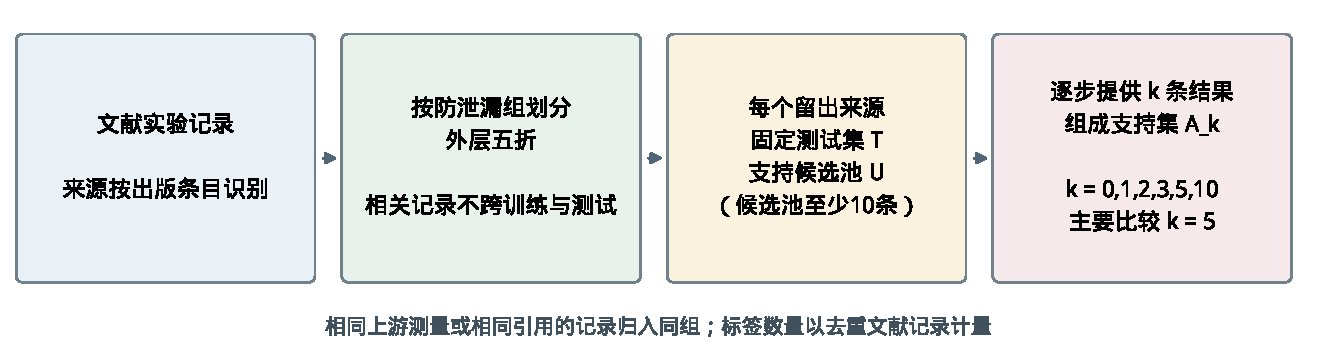
\includegraphics[width=\linewidth]{figs_cn/fig1_design.pdf}
\caption{来源隔离与少标签评估流程。先把相关记录作为整体分入外层五折，再在每个留出来源中固定测试集$T$。其余记录组成支持候选池$U$，从中逐步提供$k$条真实结果组成$A_k$。五个外层随机种子各进行一次五折评价；同一组在每个种子下恰好测试一次。各方法共享相同的测试集、支持顺序与基础模型。}
\label{fig:design}
\end{figure}

评估分为两个阶段：首先用其他文献来源训练历史基础模型；随后面对一个留出的新来源，只允许获得其中$k$条记录的真实结果，再预测该来源中固定测试集的结果。图\ref{fig:design}给出完整流程。
将最终评分的记录称为测试集$T$，其余可供选择的记录称为支持候选池$U$，实际提供结果的$k$条记录称为支持集$A_k$。扩展方法中也用$S$表示支持集、$Q$表示查询集，即待预测记录；“查询”不表示已经知道其真实结果。
标签数量设为$k\in\{0,1,2,3,5,10\}$，主要比较$k=5$，并预先指定$k=1$和$k=10$为次要比较。五条是本研究的主要比较数量，不表示已证明五次实验在经济上最优。所有分析使用已有实测记录，通过隐藏或提供其结果模拟标签获取，没有新增湿实验。

\subsection{分组交叉验证与固定测试集}
外层随机种子为$s\in\{42,101,202,303,404\}$。每个种子将防泄漏分组分成五折，轮流以一折测试、其余来源训练。同一组在每个种子下恰被测试一次。
模型选择只在外层训练来源内部进行，采用内层来源分组交叉验证，并按来源等权MAE选择配置。候选包括岭回归$\alpha\in\{0.1,1,10,100\}$，以及树数$n\in\{100,300\}$、深度$\in\{2,3\}$的梯度提升树，另保留一个较深配置。
对含$n$条记录的留出来源，不依据标签取值选取$\max(5,\lceil n/4\rceil)$条固定测试记录$T$。剩余候选池$U$随机排序，以前$k$条构成$A_k$，所以$A_1\subset A_2\subset A_3\subset A_5\subset A_{10}$。每个来源抽取50次校准顺序。
各适配方法使用完全相同的测试集、支持顺序、基础预测与外层划分。历史模型选择、先验估计和缺失值填补不使用留出来源的信息；允许提供的支持标签仅用于该来源的适配，查询标签始终只用于最后评分。

\subsection{适配方法与简单对照}
以下方法均为已有统计工具。设历史模型在支持记录上的预测为$p_A$、真实结果为$y_A$，在测试记录上的预测为$p_T$。
\begin{description}
\item[新来源均值与中位数。]分别用支持标签的平均值或中位数预测全部测试记录，不使用历史模型的预测值。它们检验仅获知来源水平能提供多少帮助，基础表中沿用“目标均值”和“目标中位数”的名称。
\item[均值偏移。]在历史预测上加$\overline{y_A-p_A}$，修正该来源的平均高估或低估。
\item[带正则化的仿射校正。]除整体偏移外，还允许修正量随中心化的历史预测发生线性变化。正则化用于限制少量支持记录下的过度拟合，其强度由训练来源确定。
\item[经验贝叶斯收缩。]将支持记录估计的偏移向历史来源折外残差所给出的先验收缩，使单条或少量标签下的修正更谨慎。
\item[局部岭回归。]用支持记录的输入与真实结果$(x_A,y_A)$重新拟合正则化线性模型，输入变换来自训练侧。这里“局部”指在当前新来源的少量记录上拟合。
\item[仅温度岭回归。]只用温度拟合支持记录，作为检验复杂输入是否具有额外价值的简单对照。
\end{description}

\subsection{误差指标与不确定性}
主要指标为来源等权平均绝对误差，简称来源等权MAE。先对每条测试记录计算预测与实测结果之差的绝对值，在同一来源内对测试记录和校准重复取平均，最后对各来源等权平均。这样，记录较多的文献不会仅因记录数多而主导评价。
对百分数响应，MAE用百分点表示。例如，实测20\%、预测22\%，绝对误差为2个百分点；它与相对误差的百分比不同。STY的MAE保留mg\,h$^{-1}$g$_{cat}^{-1}$单位。补充材料同时报告按记录加权的MAE与合并$R^2$，后者默认先平均重复预测再计算。$R^2$是相对于均值参照的平方误差指标，不表示“预测正确的记录百分比”。
不确定区间以防泄漏分组为单位进行100,000次自助重抽样，随机种子基数为510,927。区间以已拟合模型为条件，主要反映来源组之间的经验不确定性，未重新抽样整个训练流程。校准重复不作为额外独立来源。基础基准未进行多重比较校正，非主要比较保持描述性解释；后续主要选样比较使用其预定的五项比较校正。

\subsection{通过打乱对应关系检查信息作用}
基础协议包括打乱标签和打乱预测的负对照。专门的标签对应关系诊断（第\ref{sec:perm}节）对每个$A_k$进行20次均匀随机置换：支持记录和标签数值集合保持不变，只改变哪个输入对应哪个标签；每次先计算预测误差，再对置换结果平均。
因此，标签均值保持不变，而具体条件--结果关系被破坏。该分析用于回顾性地检查信息利用方式，并非正式置换假设检验，也不是实际使用时的预测规则。

\subsection{局部拟合与历史预测结构的额外作用}
扩展比较加入残差岭回归、收缩组合模型，以及依据历史数据调参的局部径向基函数（RBF）模型。RBF允许拟合非线性输入--结果关系，用于提供较强的局部对照。
记已经固定的历史模型为$f_G$，支持集为$S$，查询集为$Q$，变换后的输入为$z$。局部岭回归直接拟合$(z_S,y_S)$；残差岭回归拟合支持残差$y_S-f_G(S)$，随后将残差预测加到$f_G(Q)$上。
在相同正则化、均采用自由截距的线性拟合算子$R_{S,\alpha}$下，两种预测满足
\begin{equation}\label{eq:ext_projection}
q_R(Q)-q_L(Q)=f_G(Q)-R_{S,\alpha}[f_G(S)](Q).
\end{equation}
式中$q_R$和$q_L$分别为残差岭与局部岭预测，$R_{S,\alpha}[f_G(S)](Q)$表示把历史模型在支持点上的预测当作拟合目标，再推算到查询点。等式因此分离出历史预测中无法由该支持拟合重建的部分。研究另保留正则化完全匹配的消融，检查这一历史成分的额外价值。
收缩组合模型$q_M=(1-w)q_L+wq_R$结合两种预测。权重$w$由支持集留一预测和历史伪来源先验确定，不使用查询标签。RBF及工况、组成分块核的参数也只用允许的历史数据选择；完整定义见补充材料B。

\subsection{相同标签数量下的记录选择与输入信息交叉}
除“提供多少条结果”外，还比较“提供哪些记录的结果”。面向查询的V最优设计根据已知输入，逐步选择预计能降低查询预测工作方差的候选记录\cite{yubi,gorodetsky2016}。“工作方差”是设计模型假设下的不确定性估计，选样时不读取候选或查询的真实结果。
对照包括随机选样、覆盖选样、面向整个候选池的V选样、核V和稳健多视图V。主要选样比较固定标签数量与部署预测器参数，使差异对应于支持记录的选择。完整分析还包括历史学习的对比协方差、自适应视图选择、分块核、中心化平方或绝对风险，以及协方差平均风险等方法。
为区分组成信息对选样和预测的作用，同一个实际支持集同时交给F0和F1预测器。另一个对照只在选样程序看到的组成表中打乱整行与候选记录的对应；选中记录后，仍使用该真实记录自己的输入和实测结果拟合，查询评分也保持正确对应。此处与前节“打乱支持标签配对”的干预对象不同。

\subsection{预测权重与风险估计的敏感性}
固定自由截距的核预测器可写为$\widehat y_Q=Ay_S$，其中$A$为从支持标签计算查询预测的权重矩阵，且$A\mathbf1=\mathbf1$。
工作协方差描述设计模型假定的支持与查询响应共同变化结构。设设计时采用的工作协方差为$\Sigma_0$，实际协方差为$\Sigma$，令$B=[-A\ I]$，工作平方风险为$\mathcal R_0=|Q|^{-1}\operatorname{tr}(B\Sigma_0B^\top)$。
当$\|\Sigma-\Sigma_0\|_2\le\varepsilon$时，有
\begin{equation}\label{eq:ext_bound}
|\mathcal R_\Sigma-\mathcal R_0|\le\varepsilon\left(1+\frac{\|A\|_F^2}{|Q|}\right).
\end{equation}
这里$|Q|$为查询记录数，$\|A\|_F^2$为预测权重平方的总和。该式说明，当协方差假设存在偏差时，较强的权重放大可能增加风险估计的敏感性。它用于解释标签噪声放大和任务依赖性，不构成对实际MAE的保证。推导及惩罚项消融见补充材料B。

\subsection{不同分析流程的比较口径}
基础基准与扩展分析分别保留各自预先固定的历史拟合、适配参数和支持顺序。同一任务在不同分析流程中的未适配误差或随机选样误差，因而可能略有不同。每项收益只与同一流程中的匹配对照比较，不跨流程相减。
基础基准保留原统计口径；扩展分析的五项主要选样比较使用校正区间。其余信息干预及已经用于方法开发的实测家族分析，保持探索性或开发性解释。来源数量、随机种子数量和催化剂划分数量分别报告。

\section{结果}\label{sec:results}
\subsection{记录随机划分与陌生来源预测的差距（研究问题1）}

\begin{figure}[htbp]
\centering
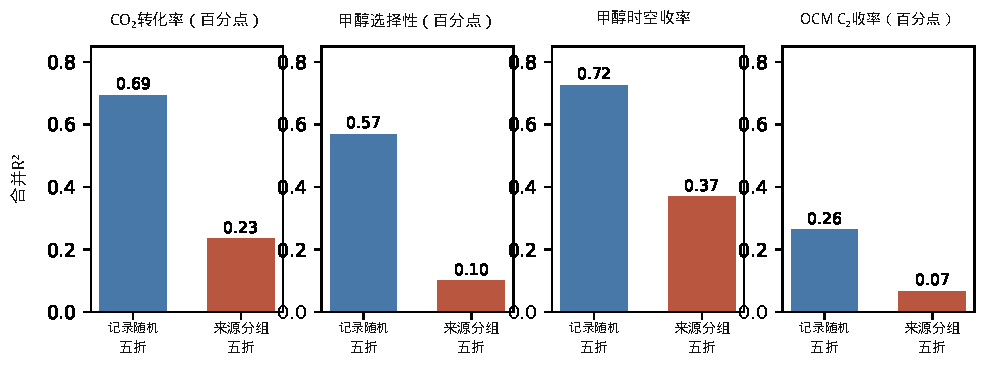
\includegraphics[width=\linewidth]{figs_cn/fig2_split_contrast.pdf}
\caption{相同记录、输入、固定模型和种子下，两种五折划分的表现。纵轴为合并$R^2$，越高越好。来源隔离相对于记录随机划分的$R^2$下降分别为0.460（转化率）、0.469（选择性）、0.356（STY）和0.196（OCM）。图中标签经过四舍五入；每条记录在每种模式、每个种子下恰好测试一次。}
\label{fig:split}
\end{figure}

在记录、输入和固定模型完全相同时，划分方式带来的变化大于本文测试的各项协变量选择差异（图\ref{fig:split}）。将防泄漏分组整体留出后，转化率、选择性、STY和OCM的合并$R^2$分别下降0.460、0.469、0.356和0.196。
记录随机划分主要评价已见来源中的新记录，来源隔离则评价陌生来源。两者对应不同任务，因此上述差值作描述性解释，不全部归因于某一种泄漏机制的因果作用。后续结果均采用来源分组划分。

\subsection{没有新来源标签时的表现（研究问题2）}
在全部合格来源的留出记录上，历史基础模型均优于仅使用历史训练均值作常数预测的对照。转化率、选择性、OCM和STY的来源等权MAE分别为5.88对6.33\pp{}、20.33对21.63\pp{}、5.47对5.82\pp{}，以及136.6对187.2\mgg{}。
能够完成整条标签数量曲线的主队列是另一来源集合，需要单独阅读。在该集合中，基础模型在转化率（5.279对5.910\pp{}）和STY（135.1对164.8\mgg{}）上更好；OCM的训练均值则略优于基础模型（5.177对5.285\pp{}）。这与第\ref{sec:repr}节所示的输入信息限制相一致，不把不同来源集合混合比较。

\subsection{增加少量新来源标签后的表现（研究问题2、3）}

\begin{figure}[htbp]
\centering
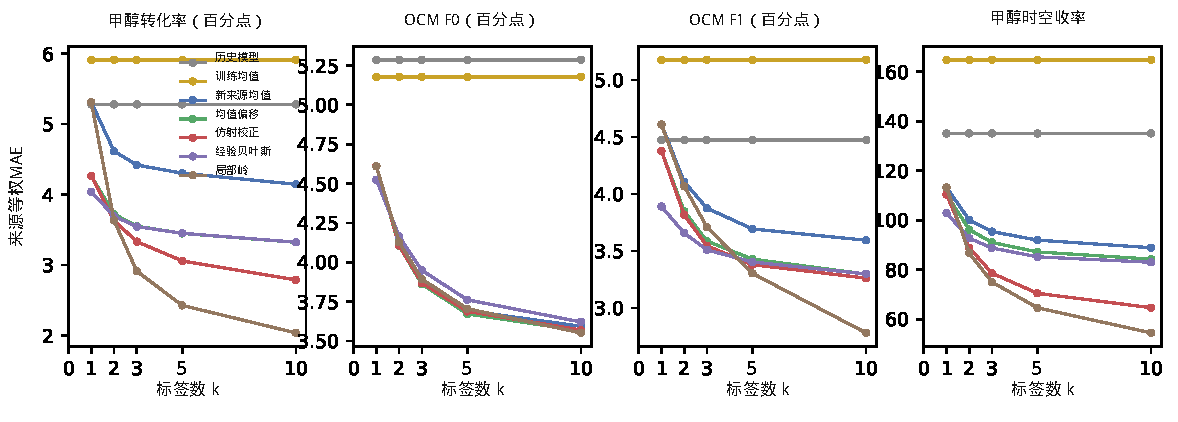
\includegraphics[width=\linewidth]{figs_cn/fig3_learning_curves.pdf}
\caption{标签数量增加时的预测误差。横轴$k$为提供的新来源真实结果数量，纵轴为来源等权MAE，越低越好；各条线表示不同方法。支持记录随机选择，$k=0$也在相同固定测试集上评价。转化率和OCM使用百分点，STY使用mg\,h$^{-1}$g$_{cat}^{-1}$，不同目标不能直接比较误差数值。}
\label{fig:curves}
\end{figure}

\begin{table}[t]
\centering\small
\caption{随机选择五条新来源标签时的平均绝对误差（MAE）。各方法使用同一测试集和相同支持记录；误差越小越好。主结果不对预测值作截断。除STY采用mg\,h$^{-1}$g$_{cat}^{-1}$外，其余目标均用百分点表示；完整95\%区间见补充材料A和数值登记表。}
\label{tab:k5}
\begin{tabular}{lcccc}
\toprule
方法 & 转化率(pp) & 选择性(pp) & OCM F0(pp) & STY \\
\midrule
历史模型（无新标签） & 5.279 & 22.736 & 5.285 & 135.115 \\
训练均值 & 5.910 & 24.167 & 5.177 & 164.803 \\
目标均值 & 4.304 & 17.136 & 3.693 & 91.993 \\
目标中位数 & 4.443 & 18.100 & 3.817 & 92.259 \\
均值偏移 & 3.450 & 15.748 & 3.672 & 87.225 \\
仿射 & 3.060 & 12.540 & 3.688 & 70.508 \\
经验贝叶斯 & 3.452 & 15.990 & 3.762 & 85.244 \\
局部岭回归 & \textbf{2.429} & \textbf{11.547} & 3.705 & \textbf{64.660} \\
\bottomrule
\end{tabular}
\end{table}
表\ref{tab:k5}与图\ref{fig:curves}给出主要标签数量及完整曲线。五条标签能够明显降低部分任务的误差，具体最优方法随任务而变。
甲醇转化率中，局部岭回归将基础MAE降低约54\%（5.28降至2.43\pp{}），仿射校正降至3.06\pp{}；STY中，局部岭回归为64.7\mgg{}，优于目标均值的92.0。
OCM-F0中，各适配方法集中在3.67--3.82\pp{}，与目标均值的差距不超过0.15\pp{}；局部岭回归为3.705，未优于目标均值3.693。因而，“新标签有帮助”与“某个方法比简单平均更好”需要分别检验。
\begin{table}[t]
\centering\small
\caption{同一来源内的方法配对比较。每格依次给出平均MAE差值和32个来源中的改善数量。差值按“方法减参照”计算，负值表示方法误差较小；括号内为改善来源数。各列分别提供1、5和10条标签，均采用随机选样。}
\label{tab:paired}
\begin{tabular}{llrrr}
\toprule
目标 & 比较 & $k=1$ & $k=5$ & $k=10$ \\
\midrule
CO$_2$转化率 & 经验贝叶斯对历史模型 & $-1.24$（21/32） & $-1.83$（23/32） & $-1.95$（24/32） \\
 & 仿射对均值偏移 & 0（构造） & $-0.39$（25/32） & $-0.53$（24/32） \\
 & 局部岭对经验贝叶斯 & $+1.27$（8/32） & $-1.02$（25/32） & $-1.29$（28/32） \\
\midrule
甲醇选择性 & 经验贝叶斯对历史模型 & $-3.87$（21/32） & $-6.75$（20/32） & $-7.20$（20/32） \\
 & 仿射对均值偏移 & 0（构造） & $-3.21$（22/32） & $-3.89$（22/32） \\
 & 局部岭对经验贝叶斯 & $+2.35$（7/32） & $-4.44$（21/32） & $-5.49$（23/32） \\
\bottomrule
\end{tabular}
\end{table}
平均误差改善也不代表每个来源都受益（表\ref{tab:paired}）。仅提供一条标签时，均值偏移使转化率的15/32个来源、选择性的17/32个来源变差；经验贝叶斯收缩将两者受损来源均降至11/32，同时未抬高平均误差。提供十条标签时，局部岭回归分别改善32/32和29/32个来源。三种$R^2$计算口径及完整方法比较（15种方法、两种选点设置和相应标签数量设置）保留于补充材料。

\subsubsection{用较强对照区分来源水平、局部关系与历史预测作用}
表\ref{tab:ext_information}将比较扩展至九类方法，并补全OCM F1。相同扩展协议下，F1的来源等权MAE从历史模型4.527降至新来源均值3.693、局部岭3.374、残差岭3.109和收缩组合3.081\pp{}。
STY中，历史模型、新来源均值、局部岭和收缩组合分别为139.258、91.993、65.210和62.608\mgg{}。
这些比较表明，少量新来源响应既可以估计整体水平，也能提供条件--结果关系。若要进一步判断历史响应结构增加了多少价值，应与使用同样标签的局部模型比较，不能把全部适配收益归于历史知识迁移。
\begin{table}[htbp]\centering\footnotesize
\setlength{\tabcolsep}{4pt}
\caption{扩展预测方法比较：随机提供五条标签。每项任务内，各方法共享支持记录和测试记录。本表采用扩展分析中预先固定的模型与支持顺序，应在表内比较；不与表\ref{tab:k5}跨表相减计算收益。STY使用原始物理单位，其余为百分点。}\label{tab:ext_information}
\begin{tabular}{lrrrrr}
\toprule
方法 & 转化率 & 选择性 & OCM F0 & OCM F1 & STY \\
\midrule
历史模型 & 5.271 & 22.740 & 5.302 & 4.527 & 139.258 \\
新来源均值 & 4.304 & 17.136 & 3.693 & 3.693 & 91.993 \\
均值偏移 & 3.455 & 15.747 & 3.672 & 3.423 & 88.265 \\
仿射校正 & 3.083 & 12.539 & 3.694 & 3.360 & 71.225 \\
经验贝叶斯偏移 & 3.457 & 15.988 & 3.759 & 3.415 & 86.510 \\
局部岭回归 & 2.429 & 11.547 & 3.655 & 3.374 & 65.210 \\
仅温度岭回归 & 2.519 & 11.535 & 3.677 & 3.677 & 87.098 \\
残差岭回归 & 2.720 & 12.077 & 3.701 & 3.109 & 69.889 \\
收缩组合 & 2.441 & 11.584 & 3.660 & 3.081 & 62.608 \\
\bottomrule
\end{tabular}

\end{table}

\subsubsection{额外来源与相同标签数量下的选样比较}
在52个能够完成完整曲线的额外文献来源中，F1历史模型、新来源均值、局部岭和收缩组合在五标签随机查询下的MAE分别为6.120、4.490、3.593和3.552\pp{}（表\ref{tab:ext_external}）。40个来源的高温查询另行报告，不与随机查询混成一个总体。
额外来源继续支持少标签条件校准的价值；出版来源的增加扩大了文献层面的证据，不能替代实验室独立性验证。
\begin{table}[htbp]\centering\footnotesize
\setlength{\tabcolsep}{4pt}
\caption{额外文献来源上的五标签预测结果。随机查询使用52个来源，高温查询使用40个来源；两类查询对象分别评价。F0和F1使用同一批实验记录。所有MAE均以百分点表示，越小越好。}\label{tab:ext_external}
\begin{tabular}{lrrrr}
\toprule
方法 & F0随机查询 & F1随机查询 & F0高温查询 & F1高温查询 \\
\midrule
历史模型 & 5.973 & 6.120 & 5.699 & 5.140 \\
新来源均值 & 4.490 & 4.490 & 5.556 & 5.556 \\
均值偏移 & 4.502 & 4.606 & 5.512 & 5.397 \\
仿射校正 & 4.284 & 4.410 & 5.209 & 5.328 \\
经验贝叶斯偏移 & 4.545 & 4.621 & 5.205 & 4.942 \\
局部岭回归 & 4.045 & 3.593 & 4.801 & 4.365 \\
仅温度岭回归 & 3.779 & 3.779 & 4.697 & 4.697 \\
残差岭回归 & 4.421 & 3.716 & 5.375 & 4.454 \\
收缩组合 & 4.054 & 3.552 & 4.806 & 4.335 \\
\bottomrule
\end{tabular}

\end{table}

固定五条标签和相同组合模型配置后，查询V选样将STY的MAE由62.608降至50.274\mgg{}，将OCM F1的MAE由3.081降至2.708\pp{}，相对于随机选样分别降低19.7\%和12.1\%（表\ref{tab:ext_acquisition}）。两项均通过原定五项任务的多重比较校正。
这说明在相应任务中，如何选择测量记录会影响同样五条结果的利用效率。其他任务的点估计与校正区间同时列出，不将全部平均改善都解释为已得到明确统计支持。
\begin{table}[htbp]\centering\footnotesize
\setlength{\tabcolsep}{4pt}
\caption{固定五条标签和相同组合预测模型配置，比较查询V选样选样与随机选样。$n$为来源数。“改善”是相对于随机选样MAE的降低比例；区间则针对原始单位下的MAE差值（查询V选样减随机），经过五项比较的多重比较校正。}\label{tab:ext_acquisition}
\begin{tabular}{lrrrrl}\toprule 预测任务 & $n$ & 随机 & 查询V选样 & 误差降低(\%) & 校正后差值区间\\\midrule
转化率 & 32 & 2.441 & 2.121 & 13.1 & [-0.707, 0.068]\\
选择性 & 32 & 11.584 & 10.683 & 7.8 & [-2.140, 0.615]\\
STY & 28 & 62.608 & 50.274 & 19.7 & [-25.965, -2.874]\\
OCM F0 & 22 & 3.660 & 3.768 & -3.0 & [-0.355, 0.714]\\
OCM F1 & 22 & 3.081 & 2.708 & 12.1 & [-0.746, -0.056]\\
\bottomrule\end{tabular}

\end{table}

\begin{figure}[htbp]
\centering
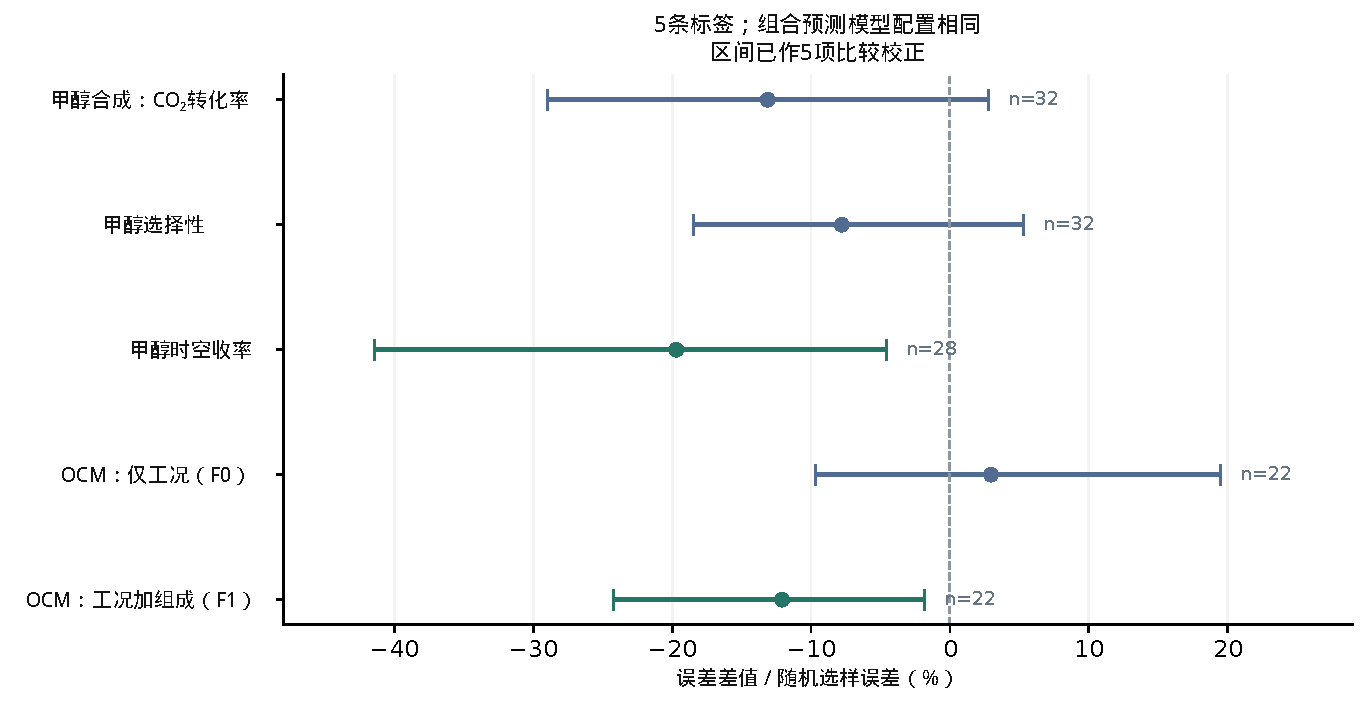
\includegraphics[width=\linewidth]{figs_cn/extension_acquisition.pdf}
\caption{五条标签、相同组合预测模型下的选样效果。圆点表示查询V相对于随机选样的MAE差值，横线表示经过五项比较校正的不确定区间；零线左侧表示查询V误差较小。为便于同图展示，各任务的差值和区间均除以该任务固定的随机选样MAE，并转成百分数。这是显示缩放，不是误差比本身的区间，也不合并不同目标的单位。}
\label{fig:ext_acquisition}
\end{figure}


在作者实测家族的固定普通查询中，采用同一个组成V支持集时，F1历史模型、新来源均值、局部岭、收缩组合和历史调参局部RBF的MAE分别为5.869、5.959、4.170、4.213和3.813\pp{}。
固定组合预测器后，组成V相对于匹配随机选样，使MAE由4.787降至4.213\pp{}，点估计降低12.0\%。局部条件模型与简单来源均值的差异支持进一步利用输入--结果关系，也表明较强的局部非线性模型应作为必要对照。


\subsection{输入信息如何影响预测与适配（研究问题4）}\label{sec:repr}
在OCM主队列的22个来源中，9个来源的所有记录具有完全相同的F0工况输入。505条记录里，391条与同来源另一条结果不同的记录共享完整六项输入。本文称这种情况为输入碰撞：模型看到的条件相同，真实结果却不同。
加入所报告组成后，主队列中输入恒定的来源数降为零，碰撞记录降至36条；在全部来源中，输入恒定的来源数由303降至168。
这种信息变化与配对误差改善一致（图\ref{fig:f0f1}）：历史模型MAE由5.285降至4.474\pp{}，差值为$-0.811$，区间为$[-1.490,-0.189]$；仿射校正改善0.309\pp{}，区间为$[-0.573,-0.063]$。
局部岭在五标签时改善0.402\pp{}，区间为$[-0.601,-0.228]$；十标签时改善0.772\pp{}，区间为$[-1.144,-0.434]$。以上区间均按F1减F0计算，负值表示F1误差较小。
两种输入设置采用相同模型选择程序，结果描述的是配对预测流程的关联，不直接证明组成的物理因果效应。F1适配后的误差仍约为3.3\pp{}，低于其未适配历史模型约4.47\pp{}，说明更丰富输入与少标签适配可以同时发挥作用。

\begin{figure}[htbp]
\centering
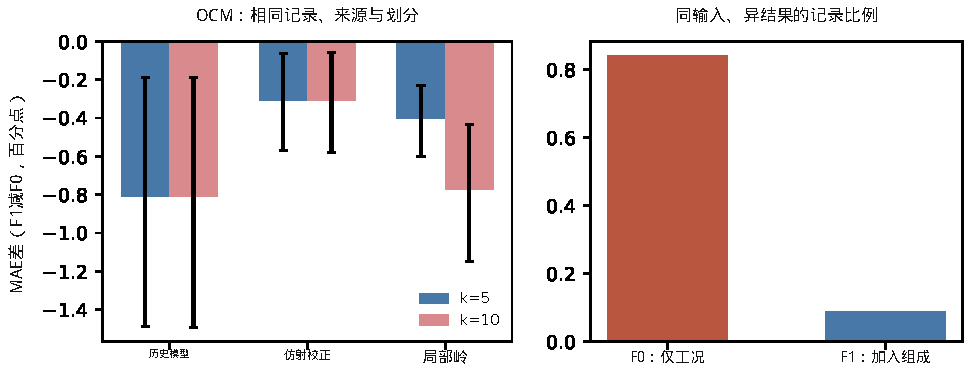
\includegraphics[width=\linewidth]{figs_cn/fig4_f0_f1_paired.pdf}
\caption{OCM中输入组成信息的配对比较。左图为F1减F0的来源等权MAE，负值表示加入组成后的流程误差较小；分别提供5条和10条标签。右图先在各来源内计算“输入完全相同、实测结果不同”的记录比例，再跨来源平均。这些记录保留在数据中，因为差异可能来自真实重复波动或未报告的条件。}
\label{fig:f0f1}
\end{figure}


\subsubsection{组成信息也可以只用于选择测量记录}
在22个历史OCM来源中，固定F0预测器、不向其提供组成信息，仅改变选样环节：组成V将组合模型MAE由匹配随机对照3.705降至3.370\pp{}。如果只打乱选样程序看到的组成行与记录身份的对应，误差回升至3.647。F1预测器下，正确组成V与打乱组成的结果分别为2.708和3.039\pp{}。
同一实际支持集同时用于F0和F1预测，因此这项交叉比较可以定位组成信息经由“选择测量记录”发挥的作用。该流程采用自己的随机支持顺序，不与其他流程的F0随机点估计跨表相减。

\begin{figure}[htbp]
\centering
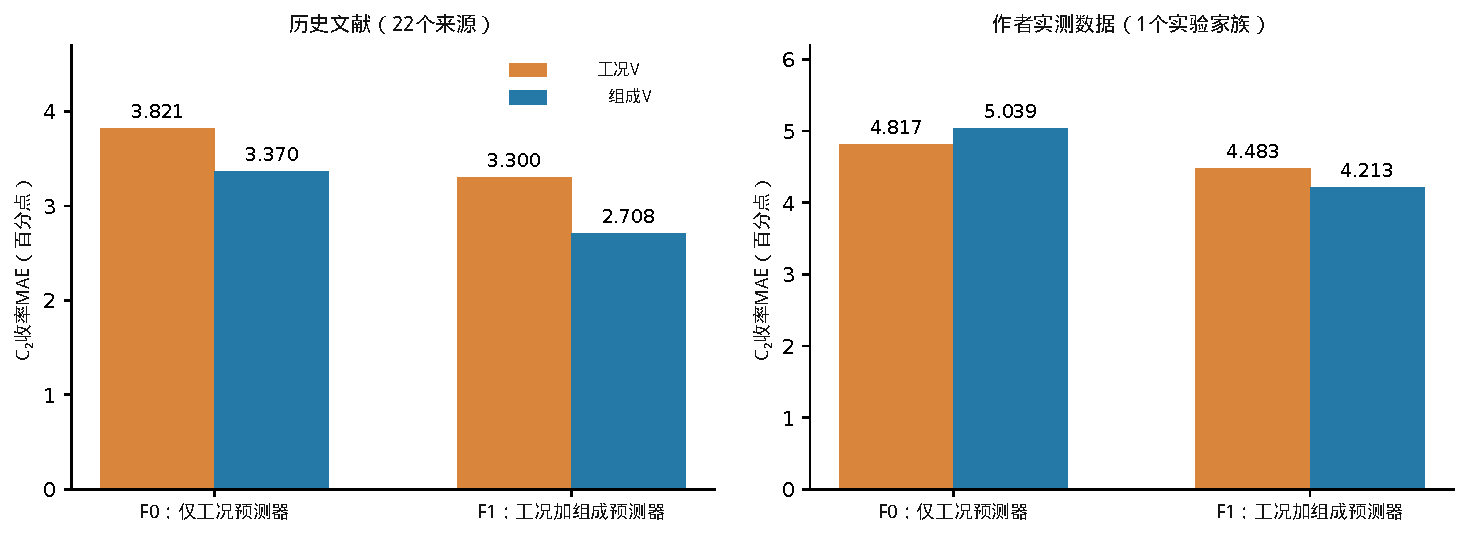
\includegraphics[width=\linewidth]{figs_cn/extension_crossing.pdf}
\caption{把选样使用的信息与预测器使用的信息分开比较。橙色为按工况选样，蓝色为按组成选样；每个选出的实际支持集同时交给F0和F1预测器。纵轴为MAE，越低越好。左、右图分别为历史文献和一个作者实测家族，显示组成信息的选样价值随预测器与来源而变。}
\label{fig:ext_crossing}
\end{figure}


在作者实测家族中，F0预测器采用工况V时优于组成V（4.817对5.039\pp{}），F1预测器则更受益于组成V。
因此，化学描述符既可能帮助拟合响应，也可能帮助安排测量；较合适的选样信息取决于预测器和待预测任务，不能只根据一种任务决定普遍排序。

\subsection{少量标签提供的是整体水平还是条件关系（研究问题3）}\label{sec:perm}

\begin{figure}[htbp]
\centering
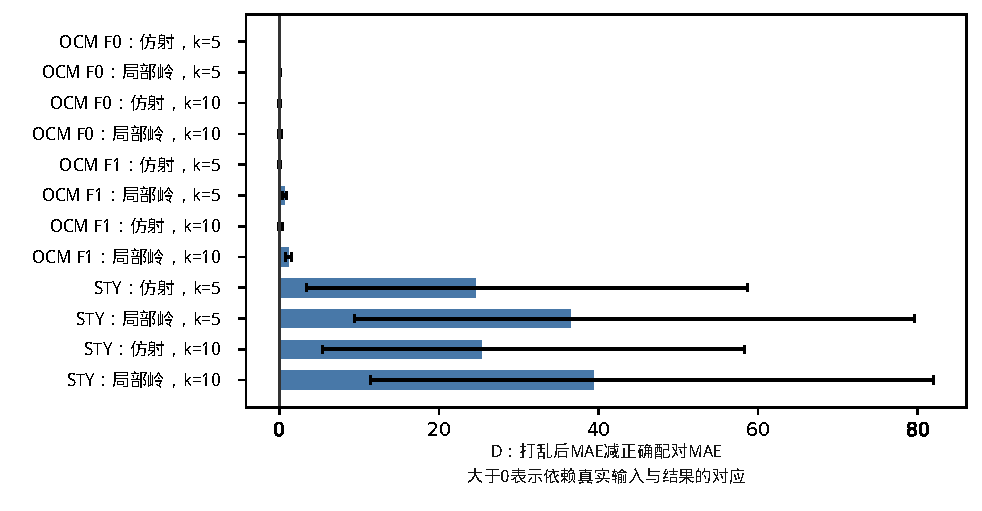
\includegraphics[width=\linewidth]{figs_cn/fig5_permutation.pdf}
\caption{标签对应关系诊断。横轴$D_{\mathrm{align}}$为“打乱标签配对后的平均MAE减正确配对时的MAE”；正值表示方法依赖真实输入与结果的对应关系。使用基准测试集分配（编号0）、校准重复0--19，每个$A_k$进行20次均匀标签置换；仿射和局部岭共享置换索引，先分别计算误差再平均。$k=1$只有一种排列，不能进行这项诊断。STY和OCM保留各自原始单位。}
\label{fig:perm}
\end{figure}

图\ref{fig:perm}通过标签置换区分两类信息。定义$D_{\mathrm{align}}$为打乱标签对应后的平均MAE减正确对应时的MAE，正值表示预测依赖正确的条件--结果配对。
OCM-F0中，仿射校正的$D_{\mathrm{align}}$为0.015，区间为$[-0.001,0.042]$。当某来源的输入完全相同时，依赖斜率的修正退化为所选标签平均水平的函数，因此在同一标签集合内部改变排列，结果可以基本不变。这里保持的是同一批标签；换成另一批记录，其均值和结果仍可能变化。
OCM-F1中，仿射诊断仍接近零，但局部岭为明确正值：五标签时为0.66\pp{}，区间$[0.44,0.90]$；十标签时为1.14\pp{}。输入包含有用组成差别后，局部岭利用了真实的输入--结果对应。
STY中，两种方法均依赖对应关系，五标签时仿射与局部岭的诊断差值分别为24.6和36.5\mgg{}。

\subsubsection{组合模型中的对应关系与历史成分}
对查询V选出的五条支持记录，保持标签数值集合和均值不变、只打乱配对，使OCM F1组合模型的MAE由2.708升至3.548\pp{}，差值为0.840，探索性条件95\%区间为$[0.478,1.237]$。
转化率、选择性和STY的相应差值分别为2.015、6.040\pp{}及30.671\mgg{}；OCM F0仅为0.047\pp{}，区间跨零（表\ref{tab:ext_alignment}）。
这些结果补充了局部岭的诊断，但不同预测器和不同支持选择规则下的差值不合并为同一个效应。
\begin{table}[htbp]\centering\footnotesize
\setlength{\tabcolsep}{4pt}
\caption{在查询V选样选出的五条支持记录上，检查标签对应关系的作用。保持支持记录、标签数值集合和均值不变，仅改变标签与输入的配对。区间为已拟合流程条件下的探索性95\%分组自助区间，未作主要比较所用的家族校正。}\label{tab:ext_alignment}
\begin{tabular}{lrrrl}\toprule
预测任务 & 正确配对 & 排列后 & MAE差值 & 95\%区间 \\ \midrule
转化率 & 2.121 & 4.135 & 2.015 & [1.253, 2.851] \\
选择性 & 10.683 & 16.723 & 6.040 & [3.693, 8.513] \\
STY & 50.274 & 80.945 & 30.671 & [10.436, 59.603] \\
OCM F0 & 3.768 & 3.815 & 0.047 & [-0.009, 0.134] \\
OCM F1 & 2.708 & 3.548 & 0.840 & [0.478, 1.237] \\
\bottomrule\end{tabular}

\end{table}

式\ref{eq:ext_projection}还用于区分局部拟合与历史响应结构的复用。F1中残差与组合模型的点估计优于局部岭，但在正则化完全匹配的历史成分消融中，各任务的区间均跨零。
因此，现有结果更直接支持新标签提供来源水平和正确配对信息；历史预测结构的额外作用，需要按任务与较强局部模型分别比较。排列观测标签的诊断也不直接识别某个化学组分的物理因果作用。

\subsection{测试集选择、排名稳定性与小来源分析（研究问题5）}\label{sec:stability}

\begin{figure}[htbp]
\centering
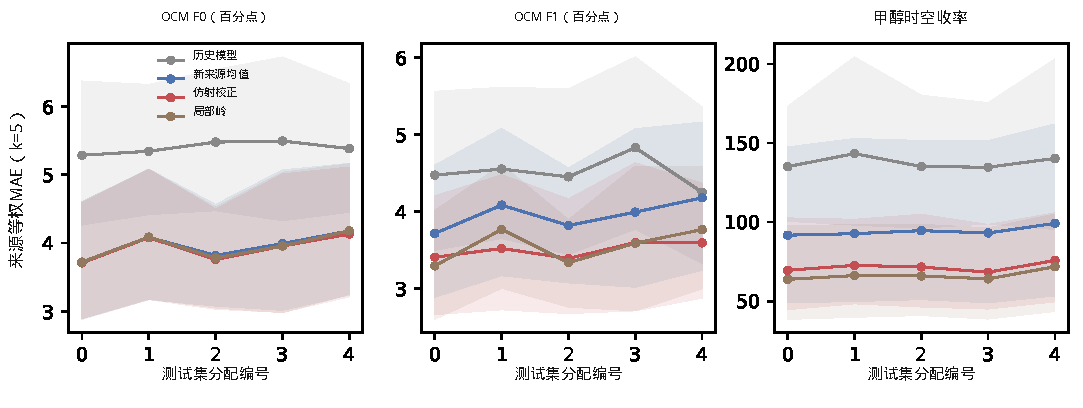
\includegraphics[width=\linewidth]{figs_cn/fig6_allocation.pdf}
\caption{固定提供五条标签，改变测试集$T$的分配。横轴0为基准分配，1--4为另外四次预先固定的分配；横轴不是标签数量。纵轴为来源等权MAE，越低越好。各方法使用相同的分配，以检查误差与排名对测试记录选择的敏感性。}
\label{fig:alloc}
\end{figure}

在基准测试集之外，再构造四种预先固定的测试集分配（图\ref{fig:alloc}）。五标签时，主队列MAE的最大移动约为0.4\pp{}（OCM）和8\mgg{}（STY）。
部分排名具有稳定性：历史模型与训练均值在各分配、各任务中均处于最后两位，STY的前两种方法（局部岭、仿射）也保持稳定。但OCM F1的局部岭排名在第1至第4之间变化，与仿射、经验贝叶斯的相对顺序依赖具体测试分配。
逐来源看，五标签仿射相对于均值偏移，在转化率、选择性、OCM F0、OCM F1和STY中分别改善25、22、8、16和23个来源，分别损害6、9、5、6和5个来源，其余为数值平局。
另设支持候选池只有3--9条记录的小来源集合，包括甲醇22、OCM 45和STY 43个来源。三标签时其定性结果相近，完整结果见补充材料；这些来源不混入主队列数字。

\subsubsection{待预测催化剂编号改变后的覆盖与稳定性}
在初始催化剂编号留出任务中，固定五条标签，并采用同一历史选择的局部RBF预测器。扩展核风险选样的MAE为3.689\pp{}，匹配随机选样和组成V分别为4.818、4.680；在同一实验家族的普通查询中，相应结果为5.145、4.792、3.813。
两个查询任务使用各自的随机对照。这说明，哪一种测量覆盖更合适，会随待预测的催化剂编号集合改变。

在20次完整催化剂编号分离划分中，组成V将RBF平均MAE由4.922降至4.107\pp{}。按两个平均误差计算，降低16.6\%，并在19/20次划分中改善（表\ref{tab:ext_repeated}）。
候选池V、扩展核风险和RBF匹配风险分别改善18、15和13次。
这一结果支持组成引导的测量覆盖在该家族编号留出任务中的稳定价值。20次划分共用测量与实验家族，既不是20个独立来源，也不能直接解释为未来成功概率95\%。
\begin{table}[htbp]\centering\footnotesize
\setlength{\tabcolsep}{4pt}
\caption{一个实测实验家族内的20次催化剂编号分离测试。各方法均提供五条标签，并采用同一个依据历史数据选定的RBF预测器。差值按“方法减同次划分的随机对照”计算，单位为百分点。“范围”表示20次划分之间的散布，不是跨独立来源的置信区间。}\label{tab:ext_repeated}
\begin{tabular}{lrrll}\toprule
选样方式 & 平均MAE & 平均差值 & 划分间差值范围 & 改善次数 \\ \midrule
随机 & 4.922 & +0.000 & +0.000 至 +0.000 & 0/20 \\
组成V & 4.107 & -0.815 & -1.616 至 +0.120 & 19/20 \\
工况V & 4.926 & +0.004 & -1.025 至 +0.731 & 11/20 \\
候选池V & 4.221 & -0.701 & -1.272 至 +0.210 & 18/20 \\
扩展核风险 & 4.480 & -0.441 & -1.545 至 +0.498 & 15/20 \\
RBF匹配风险 & 4.652 & -0.270 & -1.360 至 +0.621 & 13/20 \\
惩罚RBF风险 & 4.652 & -0.270 & -1.360 至 +0.621 & 13/20 \\
\bottomrule\end{tabular}

\end{table}

\begin{figure}[htbp]
\centering
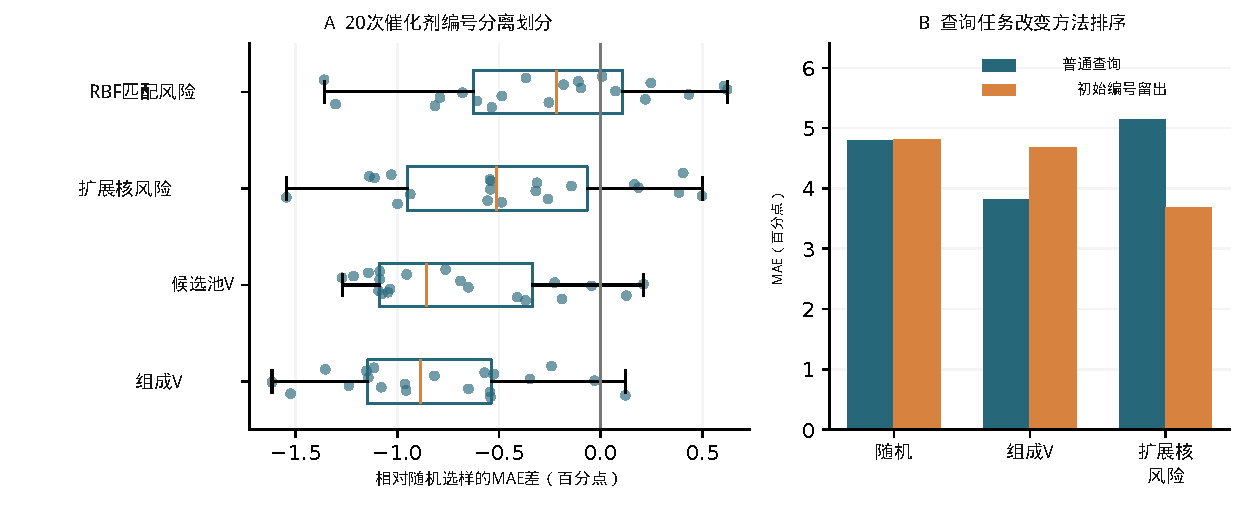
\includegraphics[width=\linewidth]{figs_cn/extension_sensitivity.pdf}
\caption{待预测对象改变时的选样表现。A展示20次催化剂编号分离划分的全部配对差值；零左侧表示优于同次随机选样。B分别展示普通查询与初始催化剂编号留出任务的MAE，越低越好。两项任务采用各自的随机对照，不能共用一个基线计算收益。}
\label{fig:ext_sensitivity}
\end{figure}


\subsubsection{固定较强预测器后比较风险目标}
在22个历史来源上，固定较强RBF预测器和五条标签，随机、组成V、扩展核风险、RBF匹配风险和惩罚RBF风险的MAE分别为3.288、2.851、2.784、2.828和2.913\pp{}（表\ref{tab:ext_risk}）。
工作风险与实际误差在来源内部的排序相关中位数为0.514，说明设计评分具有一定信息，但尚未校准为实际响应单位的误差。
25个历史外层拟合中，惩罚强度有23次选为0、2次选为0.1；在完整历史数据上选择为0。因此，式\ref{eq:ext_bound}用于解释敏感性，现有结果不支持惩罚版本普遍更优。
\begin{table}[htbp]\centering\footnotesize
\setlength{\tabcolsep}{4pt}
\caption{在22个历史来源上，固定较强RBF预测器和五条标签，比较不同选样规则。F1包含工况与组成。MAE采用百分点；工作风险是无量纲的设计评分，两者不能按数值大小直接比较。}\label{tab:ext_risk}
\begin{tabular}{lrrr}\toprule
选样方式 & MAE (pp) & 工作风险 & 放大系数 \\ \midrule
随机 & 3.288 & 0.137 & 0.563 \\
组成V & 2.851 & 0.091 & 0.583 \\
扩展核风险 & 2.784 & 0.090 & 0.627 \\
RBF匹配风险 & 2.828 & 0.090 & 0.664 \\
惩罚RBF风险 & 2.913 & 0.091 & 0.653 \\
\bottomrule\end{tabular}

\end{table}

补充材料B还保留其他开发对照。历史对比协方差预测器在线性查询V下为3.034\pp{}，其对比V为3.287，固定配置的组合模型为2.708；自适应视图选择为3.373，固定组成V为3.370，且前者在109/110个主要来源--种子组合中回退到组成视图。
协方差平均绝对风险候选未通过其五项比较校正。相同调参条件下的分块核与各向同性核、有限截距与中心化风险、平方与绝对风险，以及策略固定与重新调参的完整比较矩阵均保留。
这些对照用于判断新增机制是否带来可重复的同标签数量收益，并明确其适用条件。

\subsection{两项公开研究的复现与来源隔离复核（研究问题6）}\label{sec:audit}
为检查上述问题是否只在本文基准中出现，进一步复核两项数据与代码公开的甲醇STY研究\cite{suvarna,xu}。选择依据是公开数据、代码和逐行DOI可以恢复，与本文目标直接相关；仓库版本、数据校验值及全部计算资产均有留档。
复核关注评估设计可以支持多大范围的预测解释。Suvarna案例因原notebook的输入文件未公开，需在发布数据上进行四项有记录的兼容修改，归类为近似复现（close reproduction）；Xu的作者代码成功原样运行，归类为原流程复现（original-flow reproduction）。

\paragraph{案例一：Suvarna等的STY研究。}
作者2022年发表于\emph{Applied Catalysis B}的研究，公开仓库采用MIT许可，版本为\texttt{0dac9383}。发布数据含1,234行，每行均可映射Reference DOI；作者带输出的notebook采用随机80/20划分、种子22、训练内三折网格搜索，比较XGB、RF和GBT。
原流程近似复现（归档A层）在完整公开数据上进行兼容重建，只用于核对原随机划分结果。重新运行的XGB测试$R^2$为0.9210，作者提交结果为0.9132，差约$+0.008$；RF和GBT相应差异为$-0.007$和$+0.012$。
用于来源隔离结论的受控流程（归档B/C层）则在每个训练分区独立拟合预处理。固定记录、输入与配置，只改变划分后，相同五折下XGB的来源等权MAE由57.9升至124.0\mgg{}；按预先指定的合并预测口径，原始STY空间的$R^2$由0.876降至0.319。

\paragraph{在相同记录上比较五项与十七项输入。}
为避免跨记录集、跨测试折比较，重新在相同1,234行和相同划分上配对评价F5与F17。F5仅含温度、压力、H$_2$/CO$_2$、GHSV及SBET，不包含类别列；F17使用全部已发布描述符。
按文献来源计算配对差并进行DOI分组自助分析：记录随机划分下，F17对三个模型均有明确改善，其中XGB的MAE差为$-12.15$，区间$[-16.63,-7.42]$。
来源隔离下，GBT为$-0.05$、区间$[-13.45,+16.73]$，RF为$+2.90$、区间$[-8.72,+15.42]$，两者差异方向不确定；XGB仍有明确优势，差为$-29.56$、区间$[-42.68,-17.05]$。负值表示F17误差较低。
丰富描述符的收益依赖模型；即使XGB仍能受益，其来源隔离表现也明显低于记录随机评价。此前跨记录集、跨折的“约4个单位”比较不再作为结论，其修正过程保留于归档。

\paragraph{案例二：Xu等的STY研究。}
作者2026年发表于\emph{npj Computational Materials}的研究，仓库版本为\texttt{b7291de8}，含1,839行数据与完整预测代码。作者原流程复现（A层）的CatBoost测试$R^2$为0.8911，交叉验证为$0.8887\pm0.0121$。
来源复核使用DOI可恢复的1,757行、156个规范化来源；82条DOI缺失记录不合并成一个虚构的真实来源。
归档固定配置流程（B层）中，$\log(1+y)$空间的$R^2$为随机80/20下0.896、来源五折下0.251。这组结果保留各自划分标签。
后续严格配对比较使用相同五个种子、相同记录集及XGBoost 3.2.0配置：500棵树、深度6、学习率0.05、随机状态42。比较记录五折与DOI来源五折时，先在各来源、各种子内合并记录误差，再对来源等权平均，得到原始STY单位的MAE分别为69.6198和126.3649。
模型拟合$\log(1+y)$响应，MAE在预测值逆变换后计算。类别映射、中位数和标准化只由各训练分区确定，DOI不作为预测输入。归档随机80/20的来源等权MAE为62.9776，不与上述完整五折基线混用。
原C/D流程的嵌套选择与固定作者参数结果见补充材料A；pandas版本引起的类别列识别差异也有记录。
\begin{table}[t]\centering\small
\caption{两项公开研究的原流程复现与来源隔离复核。原流程复现单独报告；受控比较保持记录、模型配置及相应划分种子一致。MAE使用原始STY单位，$R^2$的响应空间另行注明。}\label{tab:audit}
\begin{tabularx}{\linewidth}{lXXX}\toprule
研究 & 原流程复现 & 来源隔离比较 & 比较口径\\\midrule
Suvarna 2022 & XGB $R^2$ 0.9210，作者0.9132；近似复现 & MAE 57.9$\to$124.0；$R^2$ 0.876$\to$0.319 & 匹配五折，原始STY\\
Xu 2026 & CatBoost $R^2$ 0.8911；原流程复现 & 配对复核MAE 69.620$\to$126.365 & 同五折/五种子；XGB 3.2.0；拟合log1p、MAE为原生单位\\
\bottomrule\end{tabularx}\end{table}

\begin{figure}[htbp]
\centering
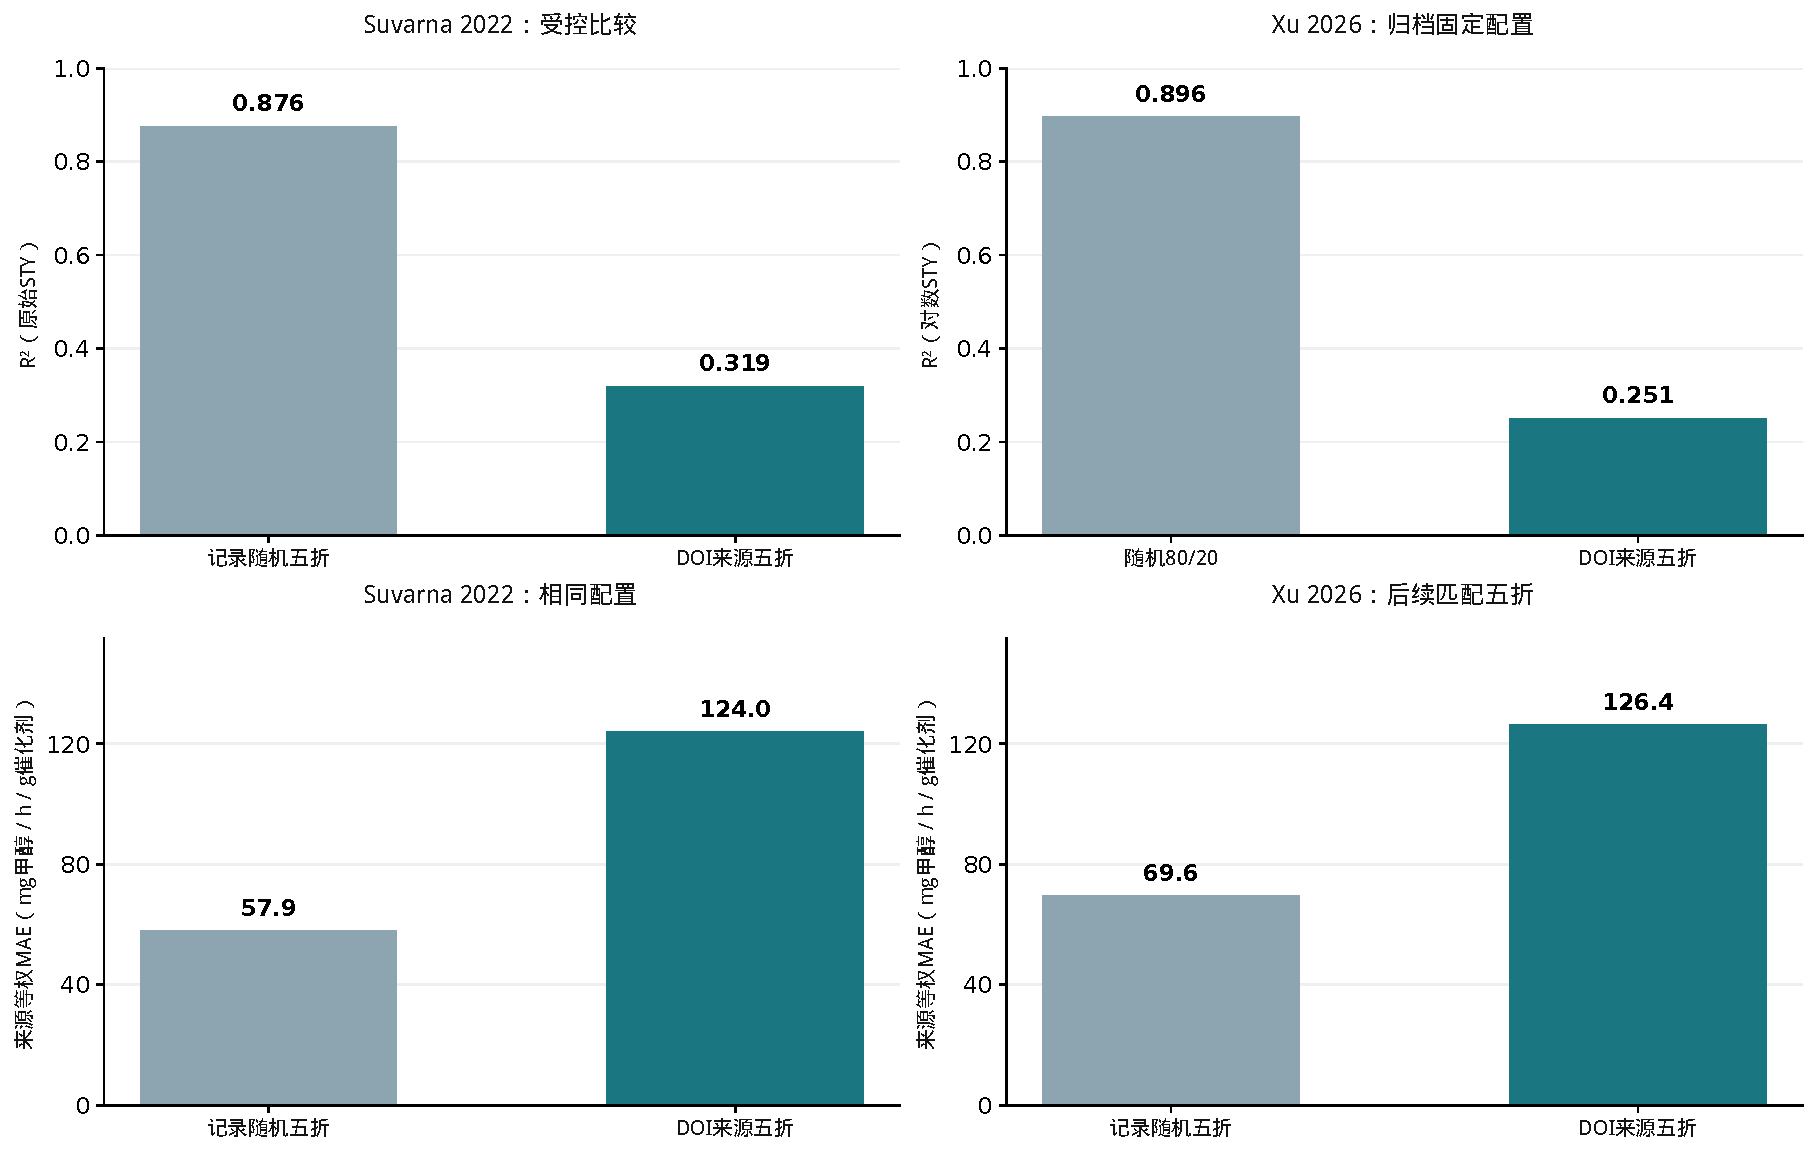
\includegraphics[width=\linewidth]{figs_cn/fig7_published_audit.pdf}
\caption{公开研究的来源隔离复核。上排为归档$R^2$，越高越好：Suvarna使用相同五折比较，Xu的归档比较分别为随机80/20与来源五折，划分形式已在横轴标明。下排为相同五折下的来源等权MAE，越低越好；Xu使用后续按来源、种子汇总的配对复核结果。原作者流程复现单独列于表中，不与其他分析流程跨层相减。}
\label{fig:audit}
\end{figure}


\paragraph{原流程成绩与陌生来源解释分别成立。}
两项研究的原流程结果均能在各自口径下恢复。陌生来源预测能力则由匹配比较单独评价：Suvarna相同五折的$R^2$为0.876降至0.319，MAE为57.9升至124.0；Xu后续相同五折、相同种子的来源等权MAE为69.6198升至126.3649，均保留对应响应单位。
不同划分的归档$R^2$及原作者流程成绩各自标注，不跨流程相减。解释来源间的批次差异，与验证陌生来源预测能力是不同目标，前者不能代替后者的直接测试。

\section{讨论}
\paragraph{把跨来源差距转化为具体的适配任务。}
来源隔离评价区分了已见文献中的新记录预测与陌生文献预测，也明确了少标签恢复所针对的差距。基础曲线和额外来源分析共同表明：在已有历史数据的基础上，获得少量新来源真实结果，可以降低该来源其余记录的预测误差。
较强局部对照和同标签数量选样进一步说明，这些测量可以提供来源水平、条件关系，以及对待预测输入的覆盖。这里讨论的是给定支持标签之后的条件预测改善；对任意未来来源完全没有标签时的表现，需要另行评价。

\paragraph{输入信息同时服务于预测和测量安排。}
OCM的F0/F1及Suvarna的F5/F17比较表明，应在相同记录与划分上评价丰富描述符的价值。选样与预测的交叉分析进一步显示，化学信息可以只用于决定先获得哪些结果，而不进入最终预测器。
STY和OCM F1的同标签数量收益，以及实测家族19/20次编号分离划分的改善，支持这一用途。待预测对象或预测器发生变化时，有价值的覆盖方式也会变化，单个支持--查询任务的排名不构成普遍排序。

\paragraph{形成可复核的评估证据链。}
岭回归、残差校准、组合、核回归和V最优设计均有成熟基础。本文的贡献是把来源隔离、标签数量、较强局部对照、信息干预和输入信息交叉比较连接起来，使预测改善及其适用条件可以检查。
公开研究复核则将原流程复现与受控划分比较分开，保留原研究在原协议下的结果，同时限定其对陌生来源的预测解释。
据此，文献催化机器学习宜同时报告记录随机与来源隔离评价；引入少标签适配时，保留使用相同新标签的局部模型及相同标签数量的选样对照。

\section{局限}
来源主要按出版条目定义，没有逐一核实实验室身份。历史数据未恢复物理制备批次，额外实测家族的报告编号也不能证明物理批次彼此独立。去重文献记录是标签数量的计量单位，不保证实验相互独立。
文献报告选择、上游来源归属质量，以及未统一的GHSV参考状态和惰性定义，仍会影响外推。组成编码只表达已报告字段，缺失不等于不存在。额外文献不重叠也不能排除共享实验室。

作者实测应用仅覆盖一个实验家族，反复划分不等于独立外部验证。历史OCM高温压力测试仅有五个合格来源。自助区间以已拟合流程为条件，未传播重新训练整个流程的不确定性；后续开发比较保留各自原有统计解释。
两项公开研究是回顾性案例，不能据此估计整个催化机器学习领域的发生比例。Suvarna属于近似复现，并非完全一致复现。工作协方差及偏差半径尚未经过真实响应风险认证。
全部结果来自既有实测记录的回顾性计算，没有新增湿实验，也未完成前瞻性自主发现验证。

\section{结论}
来源隔离评价会实质性改变对文献催化机器学习成绩的解释。少量新来源标签可以恢复部分预测表现，其信息作用可区分为来源整体水平、正确的输入--结果对应关系，以及对待预测条件的测量覆盖。
丰富输入既能帮助局部条件拟合，也能帮助决定哪些记录值得先获取结果。在相同五条标签、相同固定预测配置下，查询V相对于随机选样，使STY和OCM F1的MAE分别降低19.7\%和12.1\%。
额外文献与实测家族分析扩大了证据范围，同时表明应区分查询任务、重复划分和独立来源。两项公开研究复核继续显示，记录随机划分成绩不能自动代表陌生来源泛化。
这套按来源评价、按标签数量匹配的比较流程，为利用有限实测结果、选择适配方法和安排测量提供了可复核依据。

\section*{数据与代码可用性}
计算归档保留基础与扩展结果表、逐条记录来源、数据划分、逐行预测、固定模型及公开研究复核资产。补充材料A说明基础协议，B报告扩展方法、消融与全部比较。
上游实测数据按原始来源和再利用条款使用；本文没有新增湿实验。公共仓库标识需由作者按投稿要求提供，当前不声称已经取得仓库DOI。

\section*{复现性声明}
基础基准、公开研究复现和扩展分析分别保存软件环境、固定输入、来源与防泄漏分组、模型配置、支持顺序及结果表。各分析流程的数字均从对应归档读取。
固定RBF扩展保留2,737,000项独立实现之间的预测核对，计算结果差异低于$10^{-9}$；这表示实现一致性，不是模型对实验结果的预测误差。逐行损失、支持与查询分离，以及纳入来源的构成和数量也有相应检查。
预测条数和计算重复次数不增加独立来源数量。Suvarna的兼容修改与Xu的软件环境相关预处理差异保留原记录；近似复现和原流程复现均未改称完全一致复现。

\begin{thebibliography}{99}\small
\bibitem{toldy} Toldy, \'A. I. et al. TheMeCat: Dataset of Thermocatalytic Conversion of CO$_2$ to Methanol. \emph{Scientific Data} \textbf{13}, 165 (2026). \url{https://doi.org/10.1038/s41597-025-06482-8}.

\bibitem{yan} Yan, M. et al. A machine learning perspective on three decades of methanol synthesis: research framework and experimental operation insights. \emph{Communications Engineering} \textbf{5}, 162 (2026). \url{https://doi.org/10.1038/s44172-026-00706-4}.

\bibitem{suvarna} Suvarna, M., Ara\'ujo, T. P. \& P\'erez-Ram\'irez, J. A generalized machine learning framework to predict the space-time yield of methanol from thermocatalytic CO$_2$ hydrogenation. \emph{Applied Catalysis B: Environmental} \textbf{315}, 121530 (2022). \url{https://doi.org/10.1016/j.apcatb.2022.121530}.

\bibitem{schmack} Schmack, R. et al. A meta-analysis of catalytic literature data reveals property--performance correlations for the OCM reaction. \emph{Nature Communications} \textbf{10}, 441 (2019). \url{https://doi.org/10.1038/s41467-019-08325-8}.

\bibitem{bendavid} Ben-David, S. et al. A theory of learning from different domains. \emph{Machine Learning} \textbf{79}, 151--175 (2010). \url{https://doi.org/10.1007/s10994-009-5152-4}.

\bibitem{roberts} Roberts, D. R. et al. Cross-validation strategies for data with temporal, spatial, hierarchical, or phylogenetic structure. \emph{Ecography} \textbf{40}, 913--929 (2017). \url{https://doi.org/10.1111/ecog.02881}.

\bibitem{efron} Efron, B. \& Morris, C. Stein's estimation rule and its competitors---an empirical Bayes approach. \emph{Journal of the American Statistical Association} \textbf{68}, 117--130 (1973).

\bibitem{feudale} Feudale, R. N. et al. Transfer of multivariate calibration models: a review. \emph{Chemometrics and Intelligent Laboratory Systems} \textbf{64}, 181--192 (2002). \url{https://doi.org/10.1016/S0169-7439(02)00085-0}.

\bibitem{wu} Wu, W., Yang, M., Cheng, P. \& Wang, Y. Reliable Machine Learning Screening of Adsorption Energies Is Better Assessed with Formula-Grouped Cross-Validation. \emph{Catalysts} \textbf{16}, 742 (2026). \url{https://doi.org/10.3390/catal16080742}.

\bibitem{steyerberg2019} Steyerberg, E.\,W. \emph{Clinical Prediction Models}
(Springer, 2019).

\bibitem{mine} Mine, S. et al. Analysis of Updated Literature Data up to 2019 on the Oxidative Coupling of Methane Using an Extrapolative Machine-Learning Method to Identify Novel Catalysts. \emph{ChemCatChem} \textbf{13}, 3636--3655 (2021). \url{https://doi.org/10.1002/cctc.202100495}. Data: \url{https://github.com/mts-uw/OCM}, commit \texttt{dbf7be5aadb30323f825e8f7d7f6bd3012c99dd2}.

\bibitem{nishimura2023new} S. Nishimura, X. Li, J. Ohyama and K. Takahashi. Leveraging machine learning engineering to uncover insights into heterogeneous catalyst design for oxidative coupling of methane. Catal. Sci. Technol. 13, 4646--4655 (2023). \href{https://doi.org/10.1039/d3cy00596h}{doi:10.1039/d3cy00596h}. Author measurements: \url{https://cads.eng.hokudai.ac.jp/datamanagement/datasources/d84c1e22-ceb9-488a-8d45-4c7cf1c603b5/}.

\bibitem{yubi} K. Yu, J. Bi and V. Tresp. Active learning via transductive experimental design. ICML, 1081--1088 (2006). \href{https://doi.org/10.1145/1143844.1143980}{doi:10.1145/1143844.1143980}.

\bibitem{gorodetsky2016} A. Gorodetsky and Y. Marzouk. Mercer Kernels and Integrated Variance Experimental Design: Connections Between Gaussian Process Regression and Polynomial Approximation. SIAM/ASA J. Uncertain. Quantif. 4, 796--828 (2016). \href{https://doi.org/10.1137/15M1017119}{doi:10.1137/15M1017119}.



\bibitem{xu} Xu, W. H. et al. A natural language processing to causality framework for robust knowledge extraction of CO$_2$ hydrogenation with batch effect control. \emph{npj Computational Materials} \textbf{12}, 191 (2026). \url{https://doi.org/10.1038/s41524-026-02065-2}.


\end{thebibliography}

\end{document}
